\subsection{Spectral Energy Distribution} \label{Sec: Spectral Energy Distributions}
\subsubsection{Introduction}
The \gls{sed} of galaxies is imprinted with the effects of various physical properties influencing galaxy evolution, such as metallicity, dust, dust grain size, \gls{sf}, and \gls{agn} activity \citep{conroy_modeling_2013}. \gls{sed} analysis has grown in popularity over the years, which can be attributed to the influx of new data generated by extensive surveys, each encompassing dozens to millions of galaxies, depending on the scale and depth of the survey (some examples: \citealp{lawrence_ukirt_2007, beutler_6df_2011, desi_collaboration_desi_2016, luo_chandra_2017, barlow-hall_constraints_2023, bezanson_jwst_2024}). 

The simultaneous interaction between the aforementioned physical factors influencing galaxy evolution combines to form the total integrated spectrum, usually spanning from the \gls{uv} to \gls{fir} wavelengths. However, X-ray and radio emission can be incorporated. Dust extinction is the process in which dust absorbs the outgoing \gls{uv} radiation and re-emits in the \gls{ir} regime \citep{fu_decomposing_2010, wu_mid-infrared_2011, assef_mid-ir-_2011, han_evolution_2012}. Known as energy balance \citep{smith_panchromatic_2018}, the relative incoming spectral radiance can differentiate the total observed spectrum into their individual components.

\begin{figure}[ht]
    \centering
    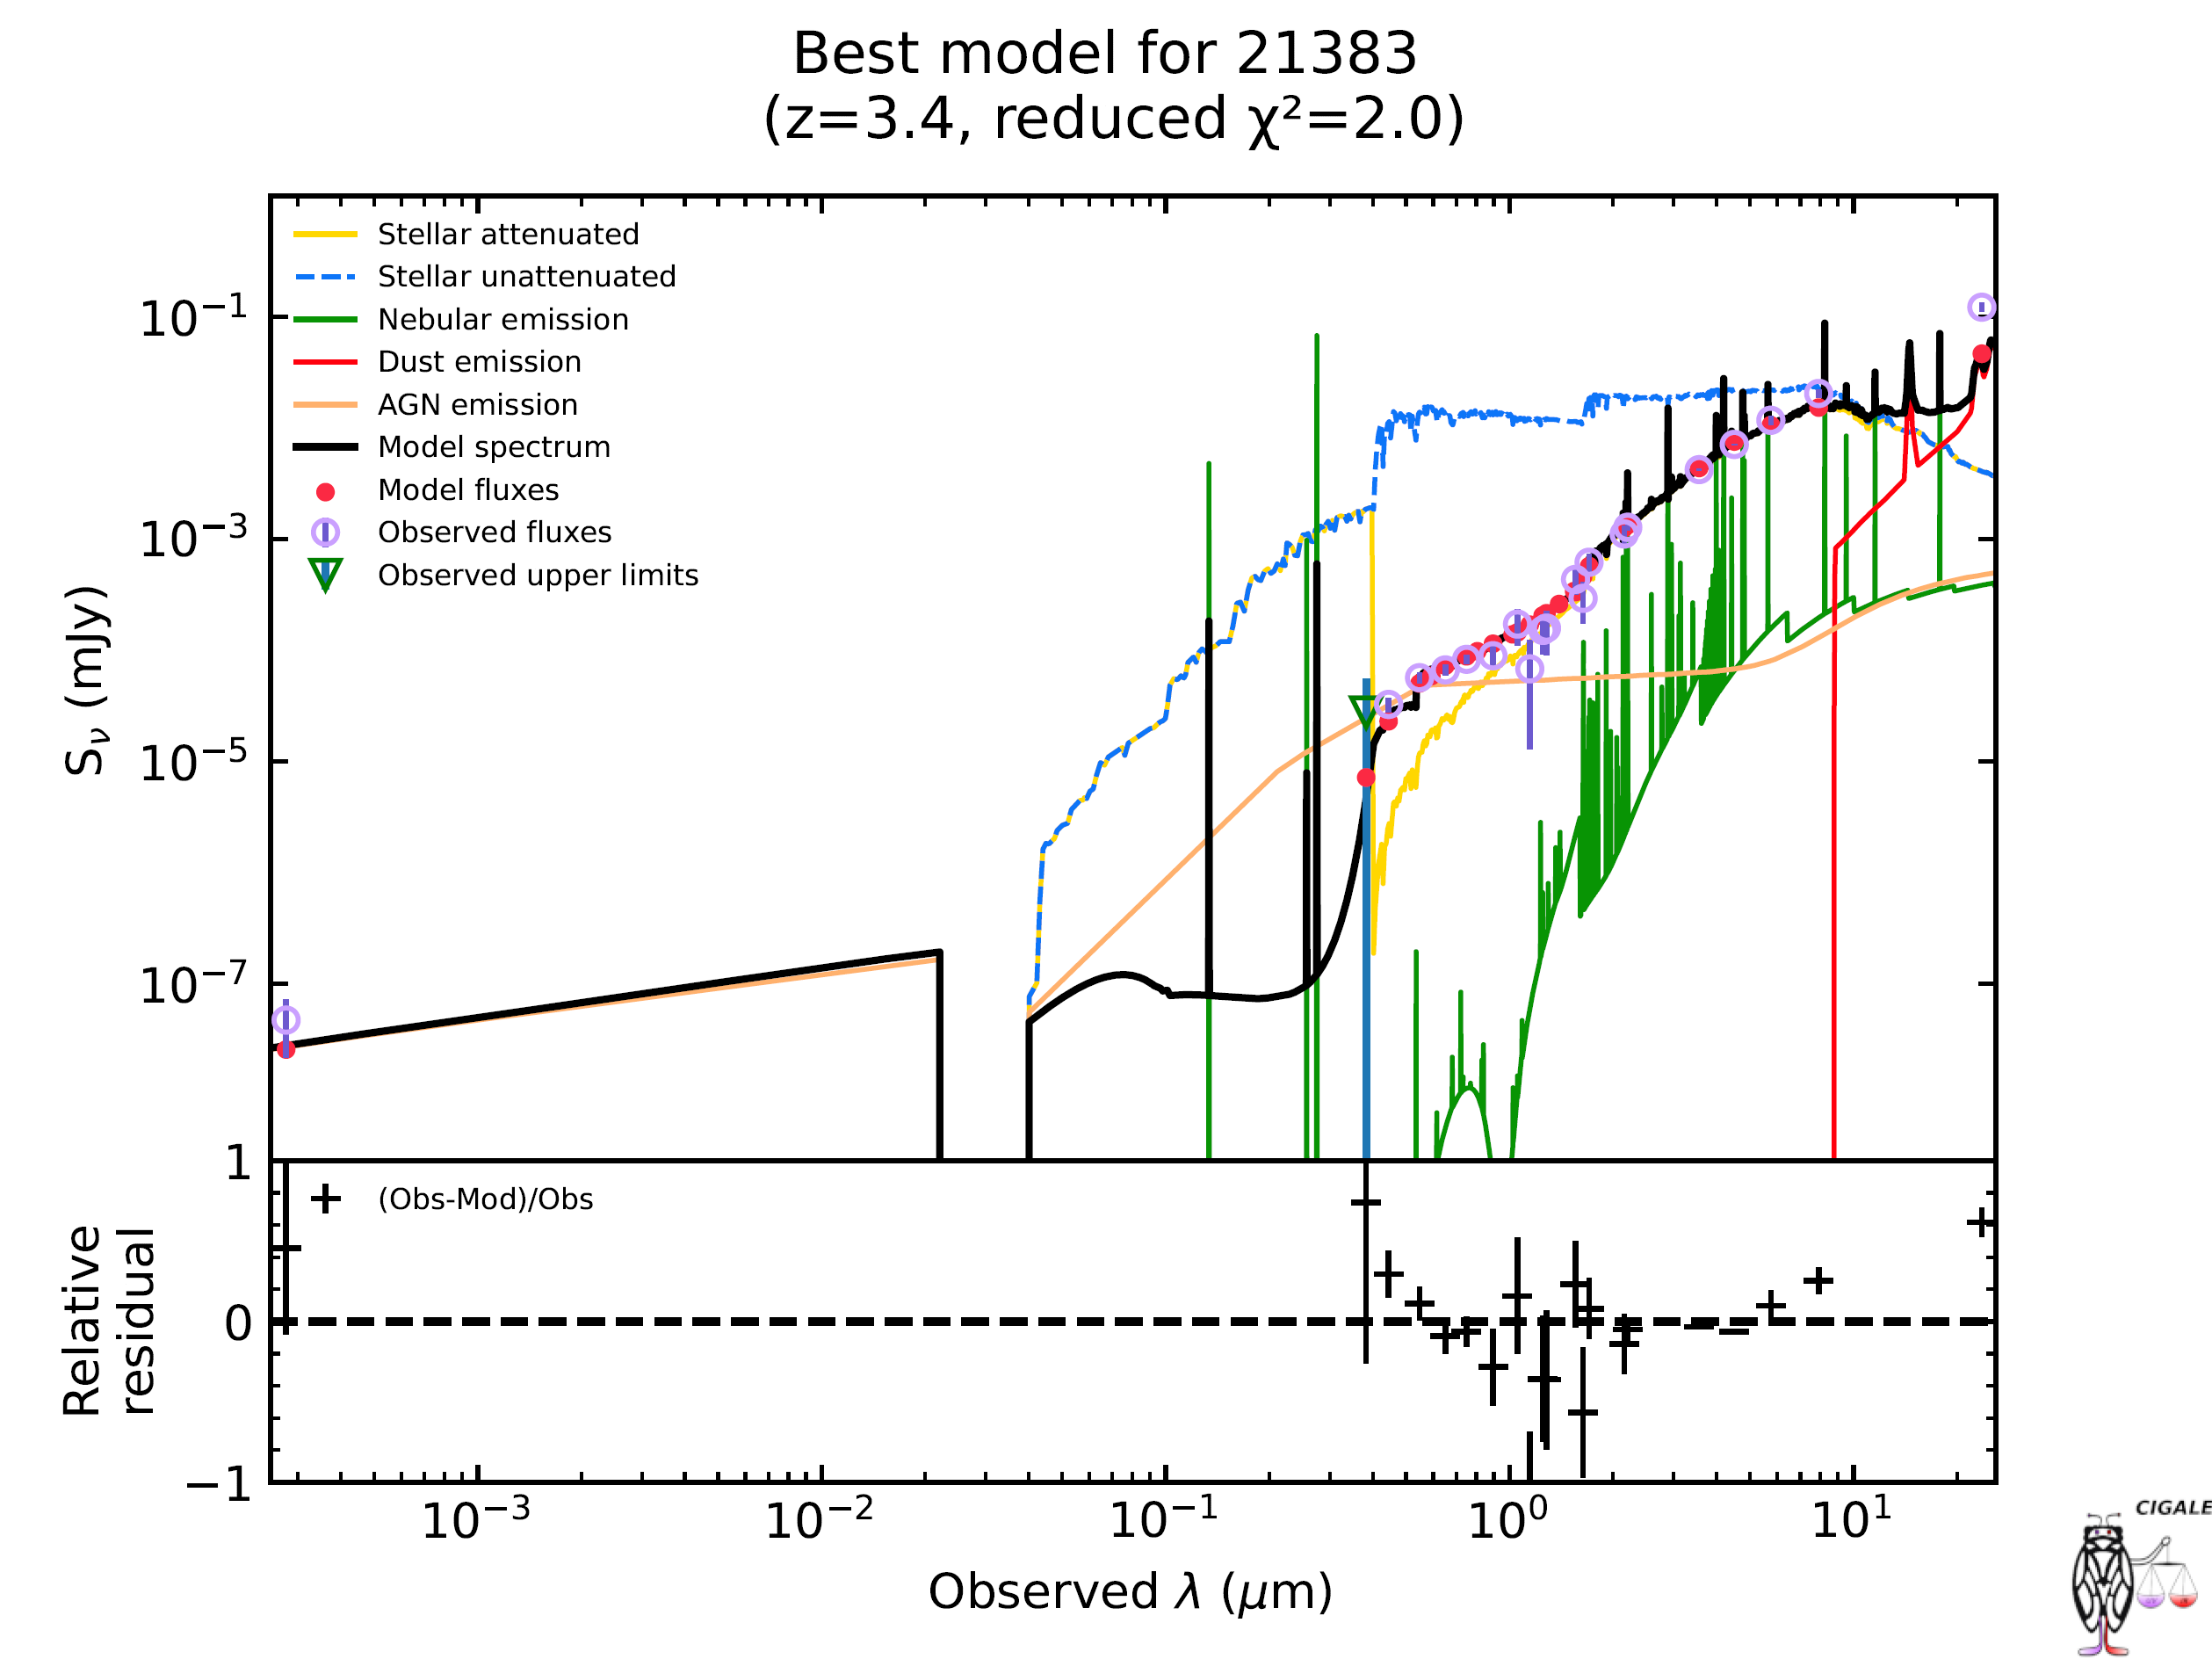
\includegraphics[width=\linewidth]{Figures/SED_Example.png}
    \caption{Example SED COSMOS-21383 ($z = 3.4$) decomposed with CIGALE ($\chi^2=2.0$) from the ZFOURGE Survey. The coloured legend in the upper left describes each line and marker. The thick black model spectrum fits the observed fluxes (purple circles). The secondary plot presents the residuals ($\chi^2$) between the model and observed data, demonstrating the fit's accuracy.}
    \label{fig: SED}
\end{figure}

\Cref{fig: SED} presents an example galaxy spectrum from the \gls{zfourge} survey \citep{straatman_fourstar_2016} which has been decomposed into individual components using \texttt{CIGALE} \citep{boquien_cigale_2019}. Each coloured element is a component of the total spectrum. Components may appear above the total black line because they are unattenuated when the total is attenuated. The template fitting is based on the observed fluxes (purple circles). The \gls{zfourge} survey aimed to observe obscured galaxies at redshifts $z>1$. This focus minimises the need for \gls{uv} wavelengths ($\lambda < \approx 1 \ \mu m$) because, as previously noted, UV light is reprocessed into the \gls{ir} range by obscuring dust and stars. Consequently, the IR range remains, which spans from $1 < \lambda < 1000 \ \mu m$. The shape of the observed \gls{sed} shifts with redshift, moving to longer wavelengths as redshift increases due to the universe's expansion. 

\subsubsection{SED Codes and Development}
Over the past two decades, new SED codes have been made available and old ones significantly upgraded, including: \texttt{MAGPHYS} \citep{da_cunha_simple_2008}, \texttt{EAZY} \citep{brammer_eazy_2008}, \texttt{ProSpect} \citep{leja_deriving_2017, robotham_prospect_2020}, and \texttt{CIGALE} \citep{boquien_cigale_2019}, among others. 

The code \texttt{EAZY} was developed to measure the photometric redshifts of faint galaxies accurately. Although \texttt{EAZY} can quantify some physical parameters, it focuses on fundamental metrics like \gls{sfr} and stellar mass, ensuring simple computations while maintaining output accuracy. \texttt{MAGPHYS} is a simple code designed to analyse complex features, including dust and gas properties, by implementing models for polycyclic aromatic hydrocarbons alongside hot and cold grains. Notably, \texttt{MAGPHYS} does not account for potential contamination from \gls{agn}, a factor that could substantially influence the accuracy and reliability of its findings. \texttt{CIGALE} is a sophisticated code to analyse various galaxy types across all wavelengths. \texttt{CIGALE} incorporates contributions from \gls{agn} and is adept at measuring various physical parameters. The methodology employed by \texttt{CIGALE} utilises composite templates that are highly versatile, allowing for tailored fitting to the diverse SEDs observed in different contexts. However, the inherent complexity of \texttt{CIGALE} also results in significant computational demands, leading to time-intensive analysis.

Numerous SED fitting codes have been developed in the literature with different purposes. These codes have yielded valuable insights into the evolution and formation of galaxies since the earliest epochs of cosmic history \citep{walcher_fitting_2011, conroy_modeling_2013}. The reader is encouraged to read \cite{thorne_deep_2022} for a brief review of \gls{sed} tools.

\subsubsection{Challenges and Limitations  Decomposition}
A challenge arises at high redshifts, as there have historically been relatively few model libraries that incorporate empirical observations. As a result, studies of high-redshift SEDs have often relied on low-redshift models to interpret their findings \citep{conroy_modeling_2013, steinhardt_templates_2023}. Discussion by \cite{haskell_energy_2023} (and authors within) has cast doubt on energy balance as a method of decomposing high-redshift galaxy \gls{sed}s due to the spatially offset emission in the \gls{uv} and \gls{ir}. In such a scenario, the \gls{uv} emission would not be absorbed and reradiated in the \gls{ir} regime, which only reduces the total derived luminosity. \cite{haskell_energy_2023} finds their successful fitting of 6706 synthetic \gls{sed}s drastically declines at $z>4$. However, their findings also show that the \gls{uv} offset does not significantly alter the derived results. Empirical templates are real \gls{sed}s observed with telescopes whereas synthetic templates are generated using theoretical models of stellar populations, dust, gas, and other physical processes \citep{hayward_should_2015, haskell_energy_2023, steinhardt_templates_2023}.

Leading work by \cite{ciesla_constraining_2015} tested \texttt{CIGALE}'s ability to estimate the physical parameters of mock galaxy \gls{sed}s when an \gls{agn} is present. They find that constraining \gls{agn} contribution is challenging when the fraction of \gls{agn} emission is less than 20\%. They also find that \gls{agn} type is a significant factor influencing the derived results with underestimation of \gls{sfr} positively correlated with Type-1 (unobscured) \gls{agn} fraction. Although Type-2 (obscured) \gls{agn} reveal discrepancies in the \gls{fir} between synthetic and empirical templates. They also find that \gls{sed}s that do not incorporate \gls{fir} data overestimate the \gls{sfr} by up to 20\%. To minimise biases, \gls{fir} data is required, and empirical templates should be utilised over synthetic templates.

As noted by \cite{hayward_should_2015}, a significant limitation of \gls{sed} modelling is the absence of empirical observations to confirm the accuracy of decomposition strategies. However, verifying these codes for every galaxy would be highly time-consuming and costly. According to \cite{silva_modelling_2011}, the computational complexity of decomposition poses challenges when handling large data sets. A more efficient and cost-effective alternative approach is synthetic \gls{sed} validation. This process involves generating mock galaxy SEDs from simulations, which can subsequently be tested using \gls{sed} codes \citep{walcher_fitting_2011, conroy_modeling_2013, hayward_should_2015, coelho_use_2020}. This method allows for the evaluation of \gls{sed} codes while mitigating the challenges associated with empirical testing; nonetheless, the scarcity of empirical observations to independently verify each component remains problematic.

As discussed by \cite{boquien_cigale_2019}, modelling the observed total SED by summating smaller components is extremely difficult because two identical SEDs can arise from vastly different physical processes. Stellar population synthesis models derive individual components to solve the degeneracy in energy balance \citep{coelho_use_2020}. This forms the basis of \gls{sed} decomposition and allows us to interpret the combination of physical factors from integrated spectra or photometry. \gls{sed} analysis is usually combined with photometry because it is time-consuming and computationally expensive. While spectroscopy provides high accuracy, it is relatively slow, whereas photometry is faster, albeit less precise.

Another challenge to overcome is that no standardised decomposition strategy in the literature exists, which exacerbates the differences between authors and their findings \citep{wu_mid-infrared_2011}. This is a problem for comparing results, as authors use different \gls{sed} codes, each with a unique design, implementation, strengths, weaknesses, priors, and input parameters and templates \citep{bellstedt_progeny_2024, mosleh_reconstructing_2025}. Authors \cite{coelho_use_2020} evaluate and discuss many limitations of \gls{sed} codes. They find that the fitting of synthetic templates leads to a worse overall fit due to inherent inaccuracies not found in empirical templates. However, they find that the choice of synthetic or empirical templates shows no significant deviation between the reddening or ages. However, empirical models with low coverage (e.g. at high redshift) can lead to underestimates of age and metallicity. 

\subsubsection{AGN Application}
Incorporating \gls{sed} decomposition into studies of galaxies is crucial for uncovering and understanding the many different evolutionary pathways galaxies and their central BHs take. As discussed in \Cref{Sec: Active Galactic Nuclei}, \gls{sf} and \gls{agn} activity directly probes galaxy evolution \citep{huang_local_2007, ho_spectral_1999, silva_modelling_2011, gruppioni_modelling_2011}. Decomposing the SED and recovering the AGN component, therefore, traces AGN coevolution with the host galaxy. 

Recent developments in SED fitting codes have opened new opportunities for uncovering fresh insights into galaxy evolution and AGN coevolution. Specifically, the introduction of higher redshift templates \citep{dale_two-parameter_2014, steinhardt_templates_2023} and templates for \gls{agn} \citep{stalevski_3d_2012, stalevski_dust_2016}. \texttt{CIGALE} \citep{boquien_cigale_2019} is one of the most advanced \gls{sed} codes available through which new and improved perspectives on the coevolution of galaxies and BHs will be attained using CIGALE's decomposition capabilities. 

In the existing literature, it is challenging to identify authors who utilise \gls{sed} codes to decompose the AGN contribution (see: \citealp{stanley_remarkably_2015, hernan-caballero_resolving_2015, cowley_decoupled_2018, brown_infrared_2019}), and even more difficult to find authors with a decomposed \gls{agn} \gls{lf} (see: \citealp{valiante_backward_2009, fu_decomposing_2010, gruppioni_modelling_2011}). This is due to the challenges of spectral decomposition, as discussed above. Among the authors who have utilised decomposition, both \cite{fu_decomposing_2010} and \cite{brown_infrared_2019} observed that the coevolution of \gls{agn} and \gls{sf} occurs simultaneously. Conversely, \cite{stanley_remarkably_2015} and \cite{cowley_decoupled_2018} find no correlation between AGN luminosity and SFR. 

\subsubsection{Conclusion}
Despite the challenges associated with \gls{sed} decomposition, \texttt{CIGALE} represents one of the most efficient and effective codes available. In this thesis, we make use of the \texttt{CIGALE} \citep{boquien_cigale_2019} \gls{sed} fitting code to generate \gls{ir} \gls{sf} and \gls{agn} \gls{lf}s of \gls{zfourge} \citep{straatman_fourstar_2016} galaxies to analyse the formation and coevolution of galaxies and \gls{agn}. \texttt{CIGALE} is likely the most sophisticated \gls{sed} decomposition code available. We standardise and streamline our methodology using the most up-to-date templates and theory to minimise the biases, limitations, and challenges associated with different decomposition techniques. How we utilise \texttt{CIGALE} to perform \gls{sed} decomposition is discussed in \cref{Sec: CIGALE}. 

% AGN activity is correlated with IR luminosity \citep{wu_mid-infrared_2011, symeonidis_what_2019, kauffmann_host_2003, symeonidis_agn_2021}, which introduces a bias against low-luminosity AGN and may help explain why AGN feedback is more prevalent at lower redshifts \citep{katsianis_evolution_2017, pouliasis_obscured_2020}.

% \subsection{Star Formation History}
% Test

% The SF fraction is also found to be a function of luminosity/redshift, decreasing as luminosity or redshift increases, while the trend is more obvious in the MIR, suggesting that the MIR wavelength is more sensitive to the presence of AGNs \cite{wu_mid-infrared_2011}. The IR-bright, dust-obscured galaxy population is crucial to understanding galaxy formation and evolution. \cite{gruppioni_modelling_2011}. IR bright galaxies emit the bulk of their energy as dust-reprocessed light generated by dusty SF or accretion onto the supermassive black holes referred to hereafter as active galactic nuclei. \cite{wu_mid-infrared_2011}

% \textcolor{red}{However, as \cite{katsianis_evolution_2017} reports, IR only works for dusty massive galaxies and is limited at higher redshifts. Less obscured (Type 1) galaxies may appear dimmer in the IR because they produce less light from reprocessing other wavelengths around the dusty torus.}

% \textcolor{red}{AGN light and star-forming (SF) light are two distinct components of the radiation emitted by galaxies. Understanding the relative contributions of these components is crucial for studying the energy sources and processes occurring within galaxies. Decomposing the spectral energy distribution (SED) into the component AGN and SF light has, until recently, rarely been performed, mostly because this was difficult to accomplish. Understanding the relative importance of AGN light and star-forming light is essential for characterising the energy sources, gas dynamics, and overall evolutionary processes occurring within galaxies. It helps in unravelling the intricate connections between supermassive black holes, galaxy evolution, and the formation of stars.}